\chapter{Introduction and Context}
\section{Overview}
The autonomous `mouse' is a design project conducted by second-year students at the University of Bath to develop their understanding of control systems and analogue circuit design. The overarching aim of the design project is to complete a lap around a 20 m track (Fig.\ref{fig:testtrack}) in the fastest time possible \cite{Robinson2025}. The `mouse' project uses differential drive achieved through two motors to navigate around, as seen in Fig.\ref{fig:mouse}.

\begin{figure}[H]
    \centering
    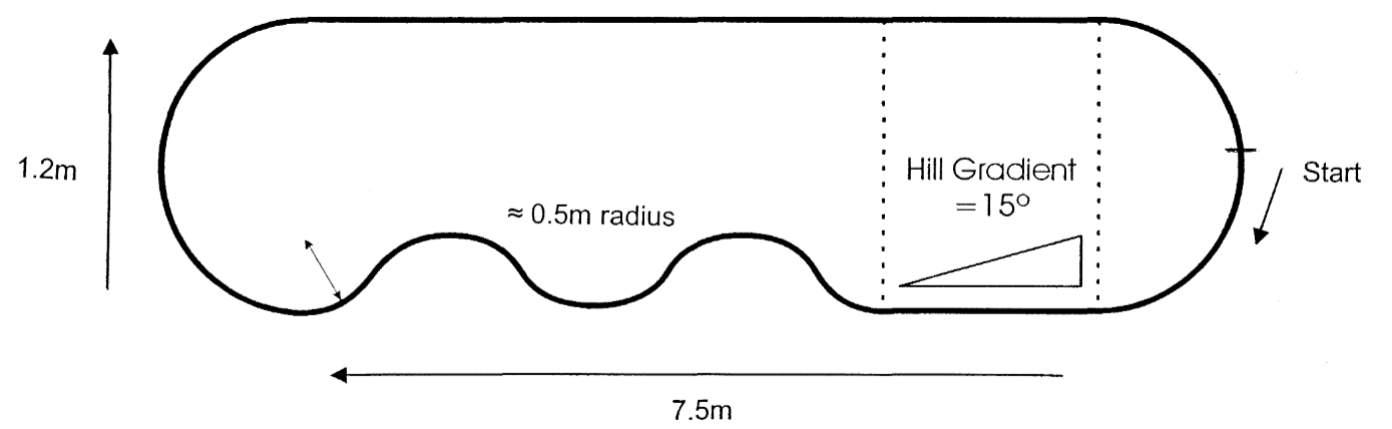
\includegraphics[width=0.9\linewidth]{photos/test_track.png}
    \caption[Mouse Track Geometry]{`mouse' test track geometry taken from \cite{Robinson2025}}
    \label{fig:testtrack}
\end{figure}

\begin{figure}[H]
    \centering
    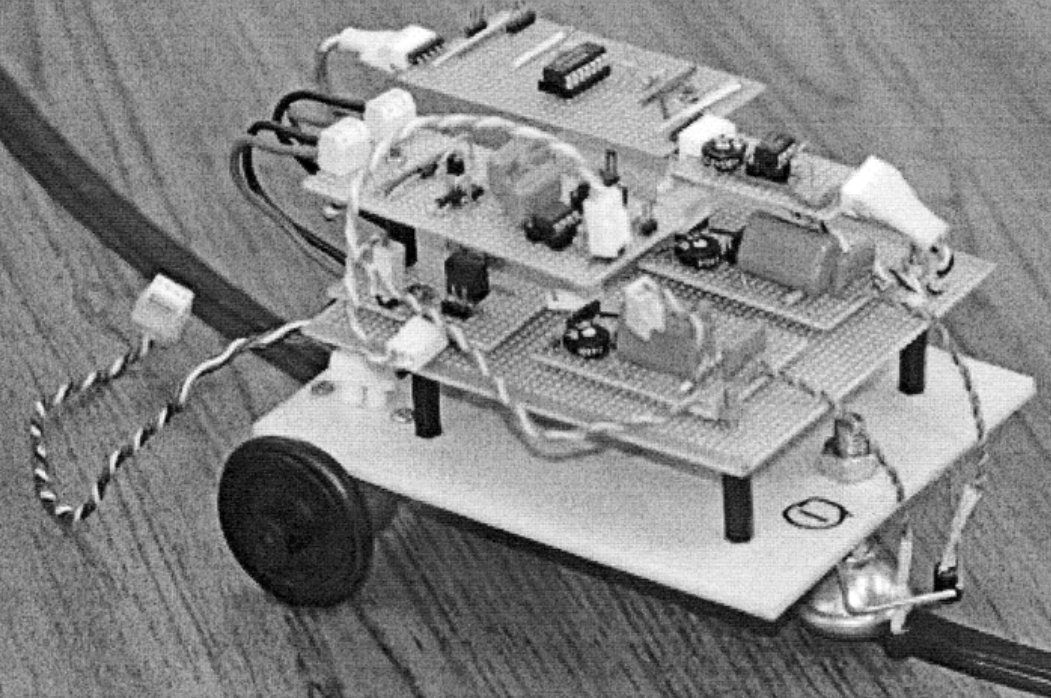
\includegraphics[width=0.6\linewidth]{photos/mouse_build.png}
    \caption[Mouse Build]{`mouse' build example taken from \cite{Robinson2025}}
    \label{fig:mouse}
\end{figure}

\newpage
The initial concepts used to design the `mouse' in the second year are described in Dr Robinson's initial document outlining the project \cite{Robinson2025}. A list of basic `mouse' building blocks can be seen below, and their integration with one another in Fig.\ref{fig:sysdiagram}.

\begin{itemize}
    \item LC filter circuit tuned to 20 kHz.
    \item Signal amplifier circuit.
    \item Peak detector.
    \item Arduino microcontroller, takes the input signal and conducts PID control to produce an output drive signal for the motors.
    \item Motor drive circuit, utilising transistors acting as switches to allow the low-power Arduino to drive the high-power motor load.
\end{itemize}

\begin{figure}[H]
    \centering
    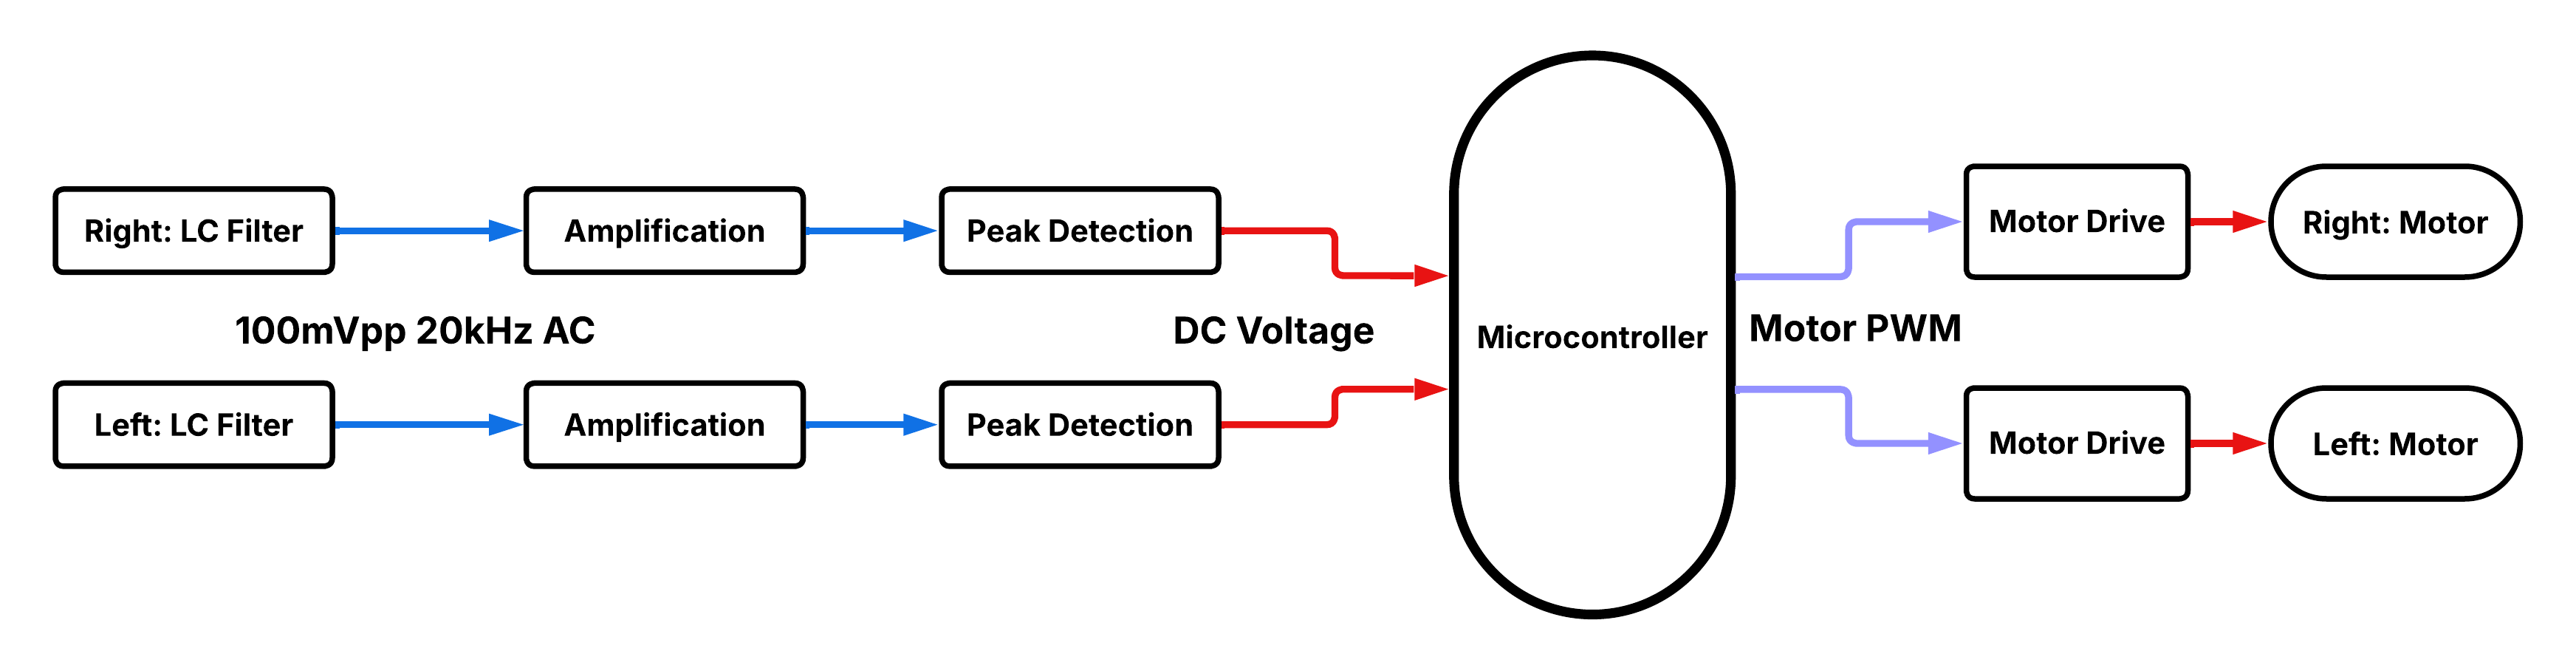
\includegraphics[width=1\linewidth]{photos/sytem diagram original.png}
    \caption[Original `mouse' System Diagram]{Original `mouse' system diagram: Blue, AC Signals; Red, DC Voltages; Purple, Digital Control Signals}
    \label{fig:sysdiagram}
\end{figure}

\subsection{Aims and Objectives}
\label{sec:aims&obj}
As previously outlined in \cite{Noah2025}, the project has three main aims with varying objectives associated with them:
\begin{enumerate}
    \item {Introduce additional stable and accurate feedback loops to the `mouse' control loop, focusing on the lack of feedback from the motors.
    \begin{itemize}
        \item Motor current.
        \item Motor speed.
    \end{itemize}}
    \item {Design alterations and suggestions for the `mouse' that are low-cost and straightforward to integrate.
    \begin{itemize}
        \item Designs should be simple to integrate into a `mouse' project and documentation be available in textbooks or data sheets to assist students if the design is harder to implement. 
        \item Component choice to be limited to low-cost components/modules, keeping a low-cost per `mouse'. Sub-system changes will ideally keep the cost within \(+25\%\) of the original cost.
    \end{itemize}}
    \item {Investigate the power supply options for the mouse, identifying methods for reducing power supply requirements.
    \begin{itemize}
        \item The number of battery packs used to power the mouse ideally reduced from 2 x \(9\) V PP3 alkaline batteries and 4 x \(1.2\) V NiMH AA batteries.
    \end{itemize}}
\end{enumerate}

\subsection{Constraints}
The constraints of this project follow those set out in \cite{Robinson2025}, with an additional self-imposed constraint of not increasing the sub-system cost by over \(25\%\) when compared to current sub-systems.

\section{Initial Ideas Regarding Implementation}
\begin{itemize}
    \item To reduce consumables, weight, and improve environmental impact by removing one of the \break \(9\) V alkaline batteries.
    \item To improve the motor control loop by adding motor current and wheel speed as additional feedback parameters. Potential new system diagram as shown in Fig.\ref{fig:completesys_block}.
\end{itemize}

\begin{figure}[H]
    \centering
    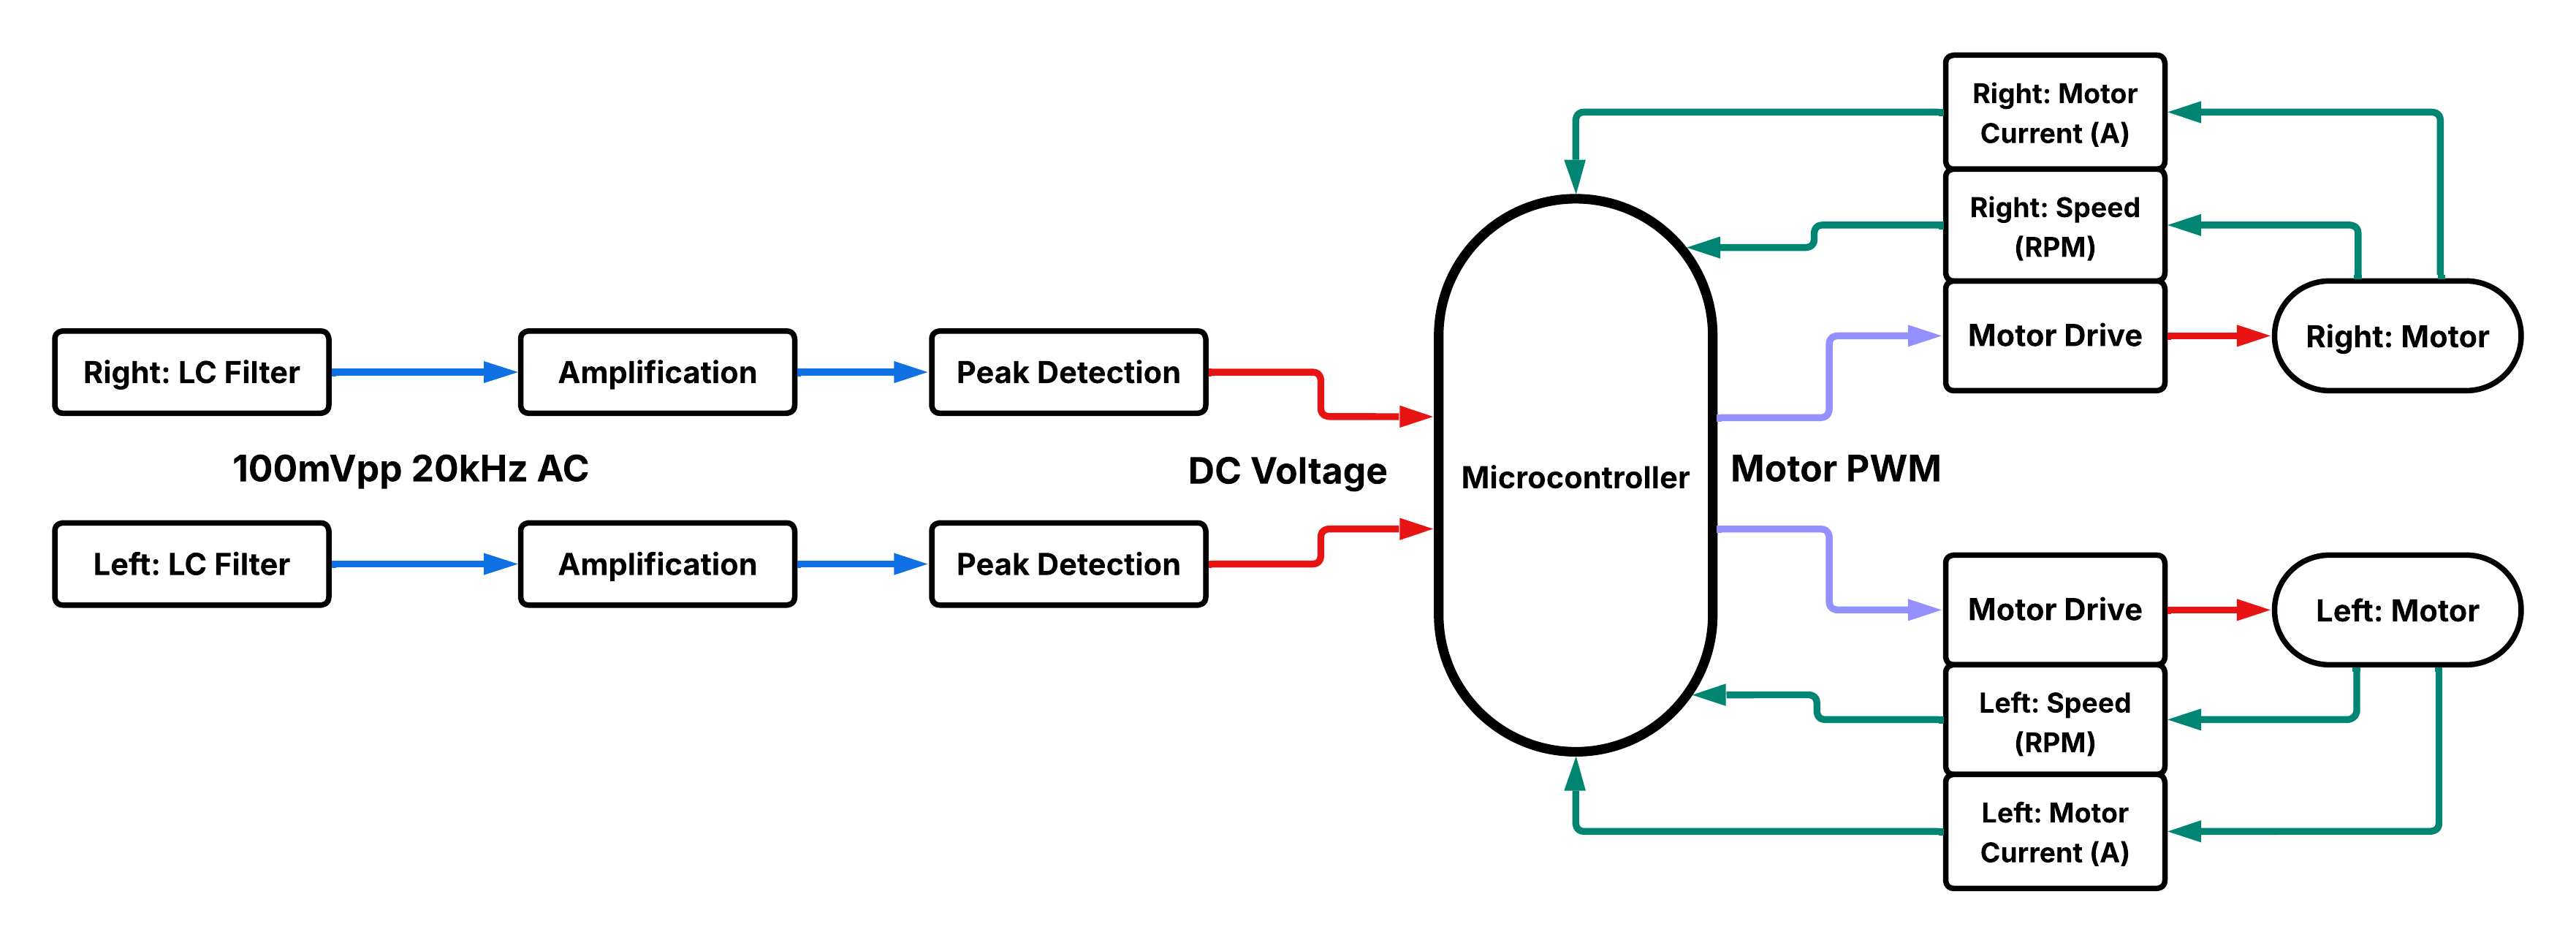
\includegraphics[width=1\linewidth]{photos/sytem diagram.png}
    \caption[Updated `mouse' System Block Diagram]{Updated `mouse' system diagram: Blue, AC Signals; Red, DC Voltages; Purple, Digital Control Signals; Teal, Additional Feedback}
    \label{fig:completesys_block}
\end{figure}


\begin{table}[H]
    \centering
    \caption{Sub-Project Letter Assignments}
    \begin{tabular}{|c|l|l|} \hline 
         \textbf{Design Letter}&   \textbf{Sub-Project Name}&\textbf{Sub-system}\\ \hline  \hline 
 \hyperref[sec:volt_div]{A}& Voltage Divider&  Position Feeedback\\ \hline
 \hyperref[sec:2]{B}& 555 Timer&Position Feeedback\\\hline
 \hyperref[sec:3]{C}& Precision Diode Clamper&Position Feeedback\\ \hline \hline 
 \hyperref[sec:4]{D}& Hall Effect Sensor&Speed Feeedback\\\hline
 \hyperref[sec:5]{E}& IR Optical Sensor&Speed Feeedback\\\hline\hline
 \hyperref[sec:6]{F}& Low Side Motor Drive&Current Feedback\\\hline
 \hyperref[sec:7]{G}& High Side Motor Drive&Current Feedback\\\hline\end{tabular}
    \label{tab:letterciruit_def}
\end{table}

Table \ref{tab:letterciruit_def} lists the sub-projects and the letters assigned for quick reference, including the relevant affected sub-systems.

\subsection{Results Gathering}
All testing procedures and methods list the equipment used, photographed in Appendix \ref{app:equip&test}.


